With the models introduced in Section \ref{chap1:sec1:ssec2}, the mean reversion in stock returns
has been examined empirically over the years. The common ground is that there are autocorrelations,
but the directions of autocorrelations are indefinite across different settings.

A brief summary is listed below, and the details are discussed in the corresponding sub-sections.

\subsection{Mean Riverse: Negative autocorrelations}\label{chap1:sec2:ssec1}
In daily, weekly and even monthly data, individual stocks have small negative autocorrelations, a.k.a., mean reverse. Mean reversion implies that
stocks are less risky for long-run investors, thus inducing investors with a longer investment horizon (e.g. younger investors, university endowments etc.) to allocate (on average)
a larger share of their portfolio to the risky asset.

Given the observation of mean reserve, if stock returns are i.i.d. over time, a mean-variance investor will choose a constant stock/bond allocation that does NOT depend on his investment horizons as a result.
In the benchmark model, investors' horizon plays no role.

Empricially, a mean-reverting component of stock prices tends to induce negative autocorrelation in returns. Several representative studies are summarized and discussed below, most of them focusing on the long-horizon returns.
I also summarize a theoretical explanation of this observation.

\subsubsection{\citet{fama1988permanent}}\label{chap1:sec2:ssec1:paper1}
Using stock returns of 1926-1985 sample period, \citeauthor{fama1988permanent} presented evidence of large negative autocorrelations for return horizons beyond a year. Their proposition is that a slowly decaying component of prices
induces negative AR in returns. This decay is slow such that for daily or weekly holding periods, it will not have a significant effect. 

\subsection{Positive autocorrelations}\label{chap1:sec2:ssec2}
Due to the positive cross-autocorrelations among individual stocks, \textbf{Stock indexes} have predominantly
positive high-frequency autocorrelations. Below, I summarize 2 papers in detail on this subject.

\subsubsection{\citet{lo1988stock,lo1990contrarian}}\label{chap1:sec2:ssec2:paper1}
\citet{lo1988stock,lo1990contrarian} presented evidence that broad market indexes have predominantly positive
high-frequency autocorrelations. In \citeyear{lo1988stock}, they found a 30\% AR(1) with weekly returns
of \textit{September 1962} to \textit{December 1985}, while higher-order ARs are also positive although smaller in magnitude.
In \citeyear{lo1990contrarian}, they found similar results with the sample period extended to \textit{December 1987}.
They proposed that the equal-weighted index autocorrelation could be rewritten into the sum of own-autocovariances
and cross-autocovariances of the component securities. Given that the autocorrelations of individual stock returns
are generally negative, they deducted that the cross-autocovariances must be positive and large enough to exceed the sum
of the negative own-autocovariances. They built the following model and showed the importance of the forecastability 
\textit{across} securities for contrarian profits:

Consider a stylized contrarian investment strategy: buy stocks at time $t$ that were losers at time $t-k$ and sell 
stocks at $t$ that were winners at $t-k$. This strategy can be formally written as 
$$
\omega_{i,t}(k)=-\frac{1}{N}(R_{i,t-k}-R_{m,t-k}),\ i=1,\cdots,N
$$
where $R_{m,t-k}=\frac{1}{N}\sum^N_{i=1}R_{i,t-k}$ is the market (equal-weighted) index return.

By construction, $\vec{\omega}_{t}(k)\equiv \left[\omega_{1,t}(k),\cdots,\omega_{N,t}(k)\right]'$ is an arbitrage portfolio 
since the weights sum to zero. Such a strategy is designed to take advantage of stock market overreactions since the stocks
whose returns deviate more from the market index return will be given higher weights (more positive for huge losers and 
vice versa). Profit generated from this strategy is $\pi_t(k)=\sum^N_{t=1}\omega_{i,t}(k)R_{i,t}$, rewrite this profit, get:

$$
\pi_t(k)= \sum^N_{i=1}\omega_{i,t}(k)R_{i,t}= -\frac{1}{N}\sum^N_{i=1}\left(R_{i,t-k}-R_{m,t-k}\right)R_{i,t} = -\frac{1}{N}\sum^N_{i=1}R_{i,t-k}R_{i,t}+R_{m,t-k}R_{m,t}
$$
take expectation, get:
\begin{align*}
    E[\pi_t(k)] &= -\frac{1}{N}\sum^N_{i=1} E\left[R_{i,t-k}R_{i,t}\right]+E\left[R_{m,t-k}R_{m,t}\right]\\
    &= -\frac{1}{N}\sum^N_{i=1}\left(Cov\left[R_{i,t-k},R_{i,t}\right] +\mu_i^2 \right) + \left(Cov\left[R_{m,t-k},R_{m,t}\right] +\mu_m^2 \right)\\
\end{align*}
where $\mu_m\equiv E\left[R_{m,t}\right]=\mu'\iota/N$. Reorganizing this equation into 3 components:
\begin{align}
    E[\pi_t(k)] &= -\frac{1}{N}tr(\Gamma_k) -\frac{1}{N}\sum^N_{i=1}\mu_i^2+\frac{\iota'\Gamma_k\iota}{N^2}+\mu_m^2 \nonumber \\
    & = \underbrace{\left\{\frac{\iota'\Gamma_k\iota}{N^2} -\frac{1}{N} tr(\Gamma_k) \right\}}_{\mathbf{L_k}}- \left\{\frac{1}{N}\sum^N_{i=1}(\mu_i-\mu_m)^2\right\} \nonumber \\
    & = \underbrace{\frac{1}{N^2}\left[\iota'\Gamma_k\iota-tr(\Gamma_k)\right]}_{\mathbf{C_k}} + \underbrace{\left(-\frac{N-1}{N}\right)tr(\Gamma_k)}_{\mathbf{O_k}} - \underbrace{\frac{1}{N}\sum^N_{i=1}(\mu_i-\mu_m)^2}_{\sigma^2(\mu)} \label{eq1.7}
\end{align}
where $tr(\cdot)$ indicates the trace operator (sum of diagonal elements).

The three components are:
\begin{enumerate}
    \item[-]: $\mathbf{C_k}$ depends ONLY on the off-diagonals of the auto-covariance matrix $\Gamma_k$
    \item[-]: $\mathbf{O_k}$ depends ONLY on the diagonals of the auto-covariance matrix $\Gamma_k$
    \item[-]: $\sigma^2(\mu)$ is independent of $\Gamma_k$
\end{enumerate}
Or, cross-autocovariances dictate $\mathbf{C_k}$, own-autocovariances dicate $\mathbf{O_k}$, this is the separation needed.

With this decomposition, the authors explained that the profitability of such a contrarian strategy could be perfectly
consistent with a \textbf{positively autocorrelated market index} and \textbf{negatively autocorrelated individual security returns}.

They also presented 5 illustrative scenarios:
\begin{enumerate}
    \item[A.] \underline{\textbf{\textit{I.I.D. returns}}}
    \begin{enumerate}
        \item[-] $\forall k, \Gamma_k=0, L_k=C_k=O_k=0$, thus, $E[\pi_t(k)]=-\sigma^2(\mu)\leq 0$. 
        \item[-] \textit{\textbf{Intuition}}: When returns do follow random walks, any cross-sectional 
        variation in expected returns would generate negative expected profits when trading with a contrarian strategy. 
        Since the strategy is reduced to shorting the higher and buying the lower mean return securities. BUT, $\sigma^2(\mu)$ is generally small.
    \end{enumerate}

    \item[B.] \underline{\textbf{\textit{Stock market overreaction}}}
    \begin{enumerate}
        \item[-] \textbf{\textit{Assumption}}: negative self-autocorrelations and zero cross-autocorrelations, i.e., 
        the diagonal elements of $\Gamma_k$ are negative, the non-diagonal elements are 0. Thus, ignoring the small $\sigma^2(\mu)$, 
        the expected profit is $$E[\pi_t(k)]\simeq L_k = O_k = -\left(\frac{N-1}{N}\right)tr(\Gamma_k) = -\left(\frac{N-1}{N}\right)\sum^N_{i=1}\gamma_{ii}(k)>0$$ 
        \item[-] \textit{\textbf{Intuition}}: In a overreacting market, "what goes up must come down" and vice versa. Thus, a contrarian investment strategy is profitable on average.
        A special case is the model of "fads": the sum of a random walk and an AR(1)\footnote{Notice that only AR(1) statisfies this conclusion.}.
    \end{enumerate}
    \item[C.] \underline{\textbf{\textit{White noise and lead-lag relations}}}
    \begin{enumerate}
        \item[-] \textbf{\textit{Assumption}}: $\forall i \in [1,\cdots,N]$, the return is given by: $R_{i,t}=\mu_i+\beta_i\Lambda_{t-i}+\epsilon_{i,t}$, where $\beta_i>0$,
        $\Lambda$ is a serially independent common factor with zero mean and variance $\sigma_{\lambda}^2$, $\epsilon_{i,t}$ is assumed to be both cross-sectionally and serially independent.
        When $k<N$, the autocovariance matrix $\Gamma_k$ has zeros in all entries except along the $k$th superdiagonal. On the $k$th superdiagonal, 
        the elements are $\gamma_{i,i+k}=\sigma^2_{\lambda}\beta_i\beta_{i+k}$, the profit is: $$E[\pi_t(k)]\simeq L_k = C_k = \frac{\sigma^2_{\lambda}}{N^2}\sum^{N-k}_{i=1}\beta_i\beta_{i+k}>0$$
        \item[-] \textbf{\textit{Intuition}}: This is an artifact of the dependence of the $i$th security's return on a lagged common factor, where the lag is determined by $i$. Notice that the returns
        are serially independent, but sotck $i$'s returns can be predicted with past returns of stock $j$, where $j<i$. With this cross-correlation, a contrarian strategy can still profit, as long
        as the cross autocovariances are sufficiently large.
    \end{enumerate} 
    \item[D.] \underline{\textbf{\textit{Nonsynchronous trading and lead-lag effects}}}\footnote{See \citet{lo1990econometric} for a detailed discussion.}
    \begin{enumerate}
        \item[-] \textbf{\textit{Assumption}}:
        
        \underline{\textit{"Virtual" return}}: the returns for security $i\in[1,\cdots,N]$ are generated by: $R_{i,t}=\mu_i+\beta_i\Lambda_i+\epsilon_{i,t}$. $\Lambda_t$ is
        some zero-mean, i.i.d. common factor, $\epsilon_{i,t}$ is zero-mean, serially and cross-sectionally independent. But this time the returns are \textit{unobservable}, i.e., "virtual".
        
        \underline{\textit{Non-trade}}: in each period $t$, security $i$ has an i.i.d. probability of $p_i$ to be NOT traded. If not traded, a security's \textit{observed} return $R^o_{i,t}$ is 0 while its
        true return is still given by $R_{i,t}=\mu_i+\beta_i\Lambda_i+\epsilon_{i,t}$. 
        
        \underline{\textit{Observed return}}: The observed return of security $i$ in period $t$ is the sum of its virtual returns of all the past \textbf{consecutive non-trading} periods.
        Formally, $R^o_{i,t}=\sum^{\infty}_{k=0}X_{i,t}(k)R_{i,t-k}$. The weights $X_{i,t}(k)\equiv(1-\delta_{i,t})\delta_{i,t-1} \cdots \delta_{i,t-k}$,
        where $\delta_i$ is the (i.i.d.) non-trading indicator. 
        $X_{i,t}(k)$ is also an indicator:
        \begin{equation*}
            X_{i,t}(k) =
              \begin{cases}
                1 & \text{$i$ is traded at $t$, but not in any of the $k$ previous periods}\\
                0 & \text{otherwise}
              \end{cases}       
          \end{equation*}
        
        \underline{\textit{Nontrading duration}}: the nontrading duration, or the number of past consecutive periods that security $i$ is not traded, 
        is $\tilde{k}_{i,t}\equiv \sum^{\infty}_{k=1}\left(\prod_{j=1}^k\delta_{i,t-j}\right)$, its expectation is $E[\tilde{k}_{i,t}]=\frac{p_i}{1-p_i}$.
        
        \underline{\textit{Portfolio return}}: for an equal-weighted portfolio of securities with common nontrading probability $p_{\kappa}$, the observed return to
        portfolio can be approximated as $R_{port,t}^o\rightarrow \mu_{port}+(1-p_{port})\beta_{port}\sum^{\infty}_{k=0}p_{port}^k\Lambda_{t-k}$, where $\beta_{port}$ is the
        average $\beta$ of the securities. Then the observed return of the portfolio over $q$ periods is $R^o_{port,T}(q)\equiv \sum^{Tq}_{t=(T-1)q+1}R^o_{port,t}$.
    
        \item[-] \textbf{\textit{Intuition}}:
        
        The "nontrading" problem aims to fix one problem: the prices of distinct securities are mistakenly assumed to be sampled simultaneously. Prices actually happen
        in different periods, but are treated as if they were observed at the same time. The "power" of a stock on others is related to how frequently it is traded: For
        a more frequently traded portfolio $a$, and a less frequently traded portfolio $b$, $R_{a,t-1}$ predicts $R_{b,t}$ better than $R_{b,t-1}$ predicts $R_{a,t}$.
        HOWEVER! This cannot fully explain the magnitude of weekly cross-autocorrelations.
    
    \end{enumerate} 
    \item[E.] \underline{\textbf{\textit{Positively dependent common factor and bid-ask spread}}}
    \begin{enumerate}
        \item[-] \textbf{\textit{Assumption:}}
        
        $R_{i,t}$ as the sum of: (a) a positively autocorrelated common factor, (b) idiosyncratic white noise, (c) a bid-ask spread process. Formally, 
        $$R_{i,t}=\mu_i+\beta_i\Lambda_i+\eta_{i,t}+\epsilon_{i,t}$$
        where $E[\Lambda_t]=0$, $E[\Lambda_{t-k}\Lambda_t]\equiv\gamma_{\lambda}(k)>0$ (positively autocorrelated common factor), $E[\epsilon_{i,t}]=E[\eta_{i,t}]=0$ (idiosyncratic noise),
        $Var[\epsilon_{i,t}]=\sigma^2_i$.

        The bid-ask spread has a AR(1) as $E[\eta_{i,t-1}\eta_{i,t}]=-s_i^2/4$, where $s_i$ is the percentage bid-ask spread. All higher-order ARs and all cross-correlations are zero.

        The autocovariance matrices are given by:
        $$\Gamma_k =
        \begin{cases}
            \gamma_{\lambda}(1)\vec{\beta}\vec{\beta}' -\frac{1}{4}diag[s_1^2,\cdots,s_N^2],&k=1\\
            \gamma_{\lambda}(k)\vec{\beta}\vec{\beta}',&k>1
        \end{cases}
        $$
        where $\vec{\beta}\equiv[\beta_1,\cdots,\beta_N]'$. The autocovariance matrices are all symmetric, which is the signature departing this model from the lead-lag process.
        The profitability is:
        $$L_k=
        \begin{cases}
            -\frac{\gamma_{\lambda}(1)}{N}\sum^N_{i=1}(\beta_i-\frac{\sum^N_{i=1}\beta_i}{N})^2 +\frac{N-1}{N^2}\sum^N_{i=1}\frac{s_i^2}{4}, & k=1\\
            -\frac{\gamma_{\lambda}(k)}{N}\sum^N_{i=1}(\beta_i-\frac{\sum^N_{i=1}\beta_i}{N})^2, &k>1
        \end{cases}
        $$

        \item[-] \textbf{\textit{Intuition:}}
        
        This model, developed by \citet{roll1984simple}, will yield a positively autocorrelated market index since the white-noise and bid-ask components will be averaged out, leaving
        the common factor $\Lambda_t$. However, for individual securities, the bid-ask spread could dominate the common factor, yielding negative autocorrelations.

        The positive profit of a contrarian strategy on returns generated by this model is solely due to the bid-ask spread (or the negative AR). In other words, if the portfolio is weighted using 
        lags 2 or higher, the strategy will only generate negative profit.
    \end{enumerate}
\end{enumerate}

With the profit decomposed in Equation \eqref{eq1.7}, \citeauthor*{lo1990contrarian} used 551 stocks that have no missing weekly returns from Jul 6, 1962 to Dec 31, 1987. They made the estimates for 
individual stocks and for 3 size-sorted quintiles. Their results can be summarized as:
\begin{enumerate}
    \item From lag 1 to even lag 4, the esimated expected profits $\hat{E}[\pi_t(k)]$ are positive. This contradicts the prediction of the common factor plus bid-ask spread model (positive only at lag 1, negative for higher lags).
    \item Although $\hat{E}[\pi_t(k)]$ is significant even at lag 4, the two components of the profits $\hat{C}_k$ and $\hat{O}_k$ are NOT significant. This suggests that $\hat{C}_k$ and $\hat{O}_k$ are negatively correlated and
    cancelling each other's noise. Since both $\hat{C}_k$ and $\hat{O}_k$ are functions of second moments and co-moments, the correlations are perhaps a result of co-skewness or kurtosis.
    \item The cross-autocorrelation matrices for the size-sorted quintiles show that current returns of smaller stocks are correlated with past returns of large stocks. This asymmetry of autocorrelation matrices implies the 
    autocovariance matrix $\Gamma_k$ is also asymmetric, contradicting the bid-ask spread model again.
    \item the cross-autocorrelation matrices also contradicts, at least partially, the non-trading model since they require an unrealistically high probability of non-trading.
\end{enumerate}

\subsubsection{\citet{froot1995new}}\label{chap1:sec2:ssec2:paper2}
\citet{froot1995new} examined the positive autocorrelations of high-frequency index returns with various market indexes and trade frequencies. The authors linked the positive correlations to an information-based explanation: slow dissemination
and inefficient processing of market-wide information. They build a simple model and show the index's theoretical autocorrelations fall with an increase in the dissemination speed of market-wide information. Furthurmore, they attribute this
decrease of positve index autocorrelations entirely to cross-stock autocorrelations. Self-autocorrelations of stocks are relatively persistent.

\noindent \underline{\textbf{\textit{A brief summary of the model}}}:
\begin{enumerate}
    \item $N$ stocks, managed by risk-neutral specialists individually. The true value is $V_t^i\equiv V_t+\xi_t^i$, where $V_i$ and $\xi_t^i$ follow independent random walks where the innovations are i.i.d. 
    normal: $\Delta V_t = u_t \sim \mathcal{N} (0,\sigma_u^2)$, $\Delta \xi_t^i =e_t^i \sim \mathcal{N}(0,\sigma_e^2)$
    \item Trading cost and technical delays of information dissemination:
    \begin{enumerate}
        \item[-] delayed observation of value: $V_t^i$ is observed at $t+1$ 
        \item[-] instant observation of order flow: $F_t^i = u_t+e_t^i+\nu_t^i$, where $u_t+e_t^i$ is an informed-traders' component, the i.i.d. $\nu_t^i \sim \mathcal{N}(0,\sigma_{\nu}^i)$ is the "liquidity" traders' component.
        \item[-] optimal price: $P_t^i=\lambda F_t^i+V_{t-1}^i$ where $\lambda=\frac{\sigma_u^2+\sigma_e^2}{\sigma_u^2+\sigma_e^2+\sigma_{\nu}^2}$ is the OLS estimator of $u_t+e_t^i$ on $F_t^i$.
        \item[-] price change from $t-1$ to $t$: $\Delta P_t^i =\lambda (u_t+e_t^i+\Delta \nu_t^i)+(1-\lambda)(u_{t-1}+e_{t-1}^i)$
    \end{enumerate}
    \item Self-autocorrelations and cross-autocorrelations:
    \begin{enumerate}
        \item[-] Self-autocovariances: $Cov(\Delta P_t^i,\Delta P_{t-1}^i)=0$
        \item[-] Cross-autocovariances: $Cov(\Delta P_t,\Delta P_{t-1})=\frac{N-1}{N}(1-\lambda)\lambda \sigma_u^2 >0$ 
    \end{enumerate}
    \item Fast market-wide information dissemination:
    \begin{enumerate}
        \item[-] $V_t$ is observable at $t$ instead of $t+1$: $V_t$ trade is costless, so traders would earn positive net profits unless innovation in $V_t$ are fully incorporated in current prices. 
        A futures market might serve as a \textit{billboard}, making the current value publicly observable.
        \item[-] optimal price: $P_t^i = \lambda^{\prime}(F_t^i-u_t)+V_{t-1}^i+u_t$, where $\lambda^{\prime}=\frac{\sigma_e^2}{\sigma_e^2+\sigma_{\nu}^2}$
        \item[-] price change of stock $i$ at $t$: $\Delta P_t^i = \lambda^{\prime}(e_t^i+\Delta\nu_t^i)+(1-\lambda^{\prime})e_{t-1}^i+u_t$
        \item[-] cross-stock autocovariances: $Cov(\Delta P_t,\Delta P_{t-1})=\frac{N-1}{N}Cov(u_t,u_{t-1})=0$, it disappears!
    \end{enumerate}
\end{enumerate}  
    
 \noindent \underline{\textit{\textbf{Empirical evidence}}}
     
\begin{enumerate}
    \item[-] \textbf{\textit{Main results}}:
    \citet{froot1995new} first examine a very short-horizon return series: 15-minute returns of S\&P 500 cash index from 1983-02 to 1989-12. They found 2 main results:
    \begin{enumerate}
        \item[1.] There are significant positive autocorrelations for 15-minute index returns.
        \item[2.] The positive autocorrelations declined/disappeared in the 1980s. 
    \end{enumerate}
\end{enumerate}

\noindent They rule out two alternative interpretations: \textbf{bid-ask bounce} and \textbf{nontrading effect} as the driving force of this decrease in autocorrelation (in other words, separate overreaction from the 
\textbf{information dissemination}).

\begin{enumerate}
    \item[-] \textbf{\textit{Bid-ask bounce}}: As described above, bid-ask bounce could lower the level of AR coefficients. In 1980s, bid-ask spread increased, leading to an increase in bounce; Investors tended to
    trade more frequently in portfolios, leading to greater synchronousness of buys and sells, leading to higher bid-ask bounce. These two facts could be linked to the decline/disappearance of the positive ARs.
    
    To rule this explanation out, \citeauthor{froot1995new} examined higher-order ARs. Bid-ask bounce would lead to equal-size reduction in all ARs, instead of just AR(1). The empirical evidence proved otherwise.
    
    They also separated bid-ask component from the last-trade index. They define $L_t$ as the index of last-trade prices and $M_t$ the index of extant midquotes for each last-trade price, the returns of them
    as $l_t=\ln(L_t/L_{t-1})$ and $m_t=\ln(M_t/M_{t-1})$. $L_t-M_t$ measures the distance between the last trade index and the log bid-ask error $l_t-m_t\simeq\Delta(L_t-M_t)$ as $\epsilon_t$. \sidenotes{$\leftarrow$ If $\epsilon_t >0$, there is a greater fraction of buys
    at time $t$ then at time $t-1$}

    $\frac{Cov(l_t,l_{t-1})-Cov(m_t,m_{t-1})}{Var(l_t)} = \frac{Cov(\epsilon_t,\epsilon_{t-1})}{Var(l_t)}+ \frac{Cov(m_t,\epsilon_{t-1})}{Var(l_t)}+\frac{Cov(m_{t-1},\epsilon_t)}{Var(l_t)}$ can be used to measure bid-ask effects. They report that the bid-ask component only
    accounts for 1/3 of the change in the AR of last trade index.
    
    When considering the three sub-components individually, they report: 
    \begin{enumerate}
        \item[-] $\frac{Cov(\epsilon_t,\epsilon_{t-1})}{Var(l_t)}$, a pure measure of Roll-type bounce, declines marginally from 1983 to 1988, while the self-autocovariance $\frac{\sum^N_i(\omega^i)^2Cov(\epsilon_t^i,\epsilon_{t-1}^i)}{Var(l_t)}$
        of the index (squared-weighted sum of self-ARs of all stocks) increases. This means that bid-ask bounce in individual stocks becomes less important and the average bid-ask spread narrows, while cross-correlation in bid-ask bounce becomes more negative and 
        portfolio trading increases. But in general, the number is too small to explain the change in the correlation of the last-trade index.
        \item[-] $\frac{Cov(m_t,\epsilon_{t-1})}{Var(l_t)}$ measures the correlation between past increases in buys/sells and current increases/decreases in the midquote index, this measure is large and positive empirically but converging to 0 over time. 2 possible explanations
        are considered:
        \begin{enumerate}
            \item[(1)] \textbf{eating-through-the-roder-book (ETOB)}: Suppose there is a limit order at the ask price and more limit orders with higher prices, then buy orders come in and deals are made firstly at the ask price and then move to higher price orders gradually.
            This way, when buy order flow is positively autocorrelated (for example, big trades are broken up and executed sequentially), an increase in buy order tends to forecast an increase in the ask price, therefore, an increase in the future midquote index.
            \item[(2)] \textbf{sluggish-response-to-roder-flow (SRFI)}: The order-flow information of a given stock is incorporated into quotes for other stocks slowly over time. For example, a buy order at the ask of GM stock (increases $\epsilon_{t-1}$) might provide incremental information
            about the value of Ford, and therefore might be associated with an increase in Ford's quotes.
        \end{enumerate}  
        The main difference between \textbf{ETOB} and \textbf{SRFI} is that ETOB is an own-stock effect, while SRFI is a cross-stock effect. And \citeauthor{froot1995new} show that \textbf{SRFI} appears to be correct, which means that bid-ask bounce cannot explain the empirical observations.
    \item[-] $\frac{Cov(m_{t-1},\epsilon_t)}{Var(l_t)}$ measures the covariance between past increases/decreases in the midquote index and current buys/sells. This statistic is negative and decreasing over time. 2 possible explanations were considered as well:
    \begin{enumerate}
        \item[(1)] \textbf{see-'em-coming (SEC)}: specialists expect the upcoming order flow and raise/reduce prices as buy/sell orders arrive (bid-ask prices rise/fall as buy/sell orders peak locally, therefore $m_{t-1}$ and $\epsilon_t$ are negatively correlated).
        \item[(2)] \textbf{slow-responce-to-price-information (SRPI)}: some stocks' quoted prices respond slowly to information (sticky), when the quickly-responding stocks trade at higher/lower quote prices, the "sticky" stocks' quoted prices remain the same. Smart investors will buy/sell these sticky stocks to profit.
    \end{enumerate} 
    Once again, SEC is an own-stock effect while SRPI is a cross-stock effect. Emperically, the authors proved that SRPI appears correct.
    \end{enumerate}
    In summary, \citeauthor{froot1995new} proved that bid-ask effects only account for 1/3 of the decline of AR. of this 1/3, nearly 1/2 might be attributed to slow-responce-to-information hypotheses (SRFI and SRPI).
    
    \item[-] \textbf{\textit{Nontrading}}: They examined two factors of the non-trading effect: trade frequency and degree of synchronousness. They calculated a measure of \textit{staleness}: the difference between last-trade midquote $m_t$ and the \textit{current} midquote $cm_t$: $m_t = cm_t+s_t = cm_t+(m_t-cm_t)$,
    where $cm_t$ is the return on the current midquote index, free of staleness and bid-ask bounce. Empirically, the decline of AR of $cm_t$ is greater than that of $m_t$, which means that nontrading staleness does NOT explain the reduction of index's AR.

    Define equally-weighted current midquote index as $eq_t$ (versus value-weighted index $cm_t$) and $z_t = cm_t-eq_t$, then decompose the autocovariance of $cm_t$, get:
    $\frac{Cov(cm_t,cm_{t-1})}{Var(l_t)}=\frac{Cov(eq_t,eq_{t-1})}{Var(l_t)}+\frac{Cov(eq_t,z_{t-1})}{Var(l_t)}+\frac{Cov(z_t,eq_{t-1})}{Var(l_t)}+\frac{Cov(z_t,z_{t-1})}{Var(l_t)}$, loosely speaking, the four items on the right-hand side can be seen as a predictability matrix:
    
    \begin{center}
        \begin{tabular}{cccc} 
        \hline
        & & \multicolumn{2}{c}{Predictee} \\
        & &small stocks & large stocks\\
        \hline
        \multirow{2}{4em}{Predicter} & small stocks & $\frac{Cov(eq_t,eq_{t-1})}{Var(l_t)}$ & $\frac{Cov(z_t,eq_{t-1})}{Var(l_t)}$ \\ 
        & large stocks & $\frac{Cov(eq_t,z_{t-1})}{Var(l_t)}$ & $\frac{Cov(z_t,z_{t-1})}{Var(l_t)}$ \\ 
        \hline
        \end{tabular}
    \end{center}

    If stocks respond symmetrically to market-wide information, the decline in the AR of $cm_t$ would be distributed equally across the four components. However, the authors showed than the decline in AR of $cm_t$ was driven by $\frac{Cov(eq_t,eq_{t-1})}{Var(l_t)}$ and $\frac{Cov(z_t,eq_{t-1})}{Var(l_t)}$,
    in other words, it has become more difficult to predict small stocks' returns, no matter with other small stocks' returns or large stocks' returns. 
    
    To incorporate information dissemination, consider $\frac{Cov(m_t,m_{t-1})}{Var(l_t)}-\frac{Cov(cm_t,cm_{t-1})}{Var(l_t)} = \frac{Cov(s_t,s_{t-1})}{Var(l_t)}+\frac{Cov(s_t,cm_{t-1})}{Var(l_t)}+\frac{Cov(cm_t,s_{t-1})}{Var(l_t)}$, where $s_t$ is the new information in quotes beyond that reflected in the trade. They found that
    the changes of both $\frac{Cov(s_t,s_{t-1})}{Var(l_t)}$ and $\frac{Cov(s_t,cm_{t-1})}{Var(l_t)}$ are negligible, while $\frac{Cov(cm_t,s_{t-1})}{Var(l_t)}$ was negative and rising over time, which means the responsiveness of current quotes ($cm_t$) to information between $t-1$ and the last trade as of time $t-1$ ($s_{t-1}$) declines,
    the evdience of more rapid dissemination of market-wide information.
\end{enumerate}

With market excess return data from \href{https://mba.tuck.dartmouth.edu/pages/faculty/ken.french/data_library.html}{Kenneth French's website}, I replicate the AR(1)s of daily value-weighted market index returns from 1926 to 2021\footnote{As documented on Kenneth French's website, the market return consists of all CRSP firms incorporated in the US and listed on the NYSE, AMEX, or NASDAQ with a CRSP share code of 10/11}.
The autocorrelations are estimated in a rolling window of 300 trading days. The time series of AR(1) coefficients is shown in Figure \ref{fig1-1}. The daily ARs of the market returns were positive till late 1990s, but the decline started from 1970s. Negative daily ARs are observed in recent years (since mid-2000s). 

\begin{figure}[ht]
    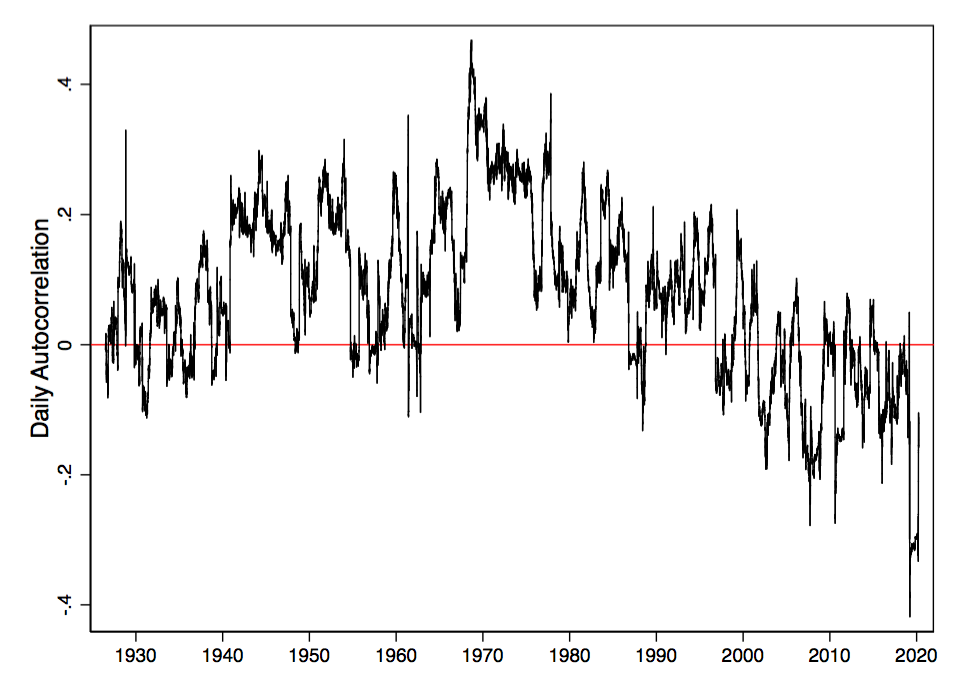
\includegraphics[width=14cm]{fig1-1.png}
    \centering
    \caption{Daily Autocorrelation of the Excess Market Return, 1926-2021}\label{fig1-1}
\end{figure}